% Drawing 86/01-2 -- folder 86, batch 01, archive page 18 (PDF page 19).
% Transcription: en marge gauche, un croquis : l'arête $a = \{s, t\}$, les sommets $u$, $v$, et les quatre sommets $\Pi_{s,u}$, $\Pi_{s,v}$, $\Pi_{t,u}$, $\Pi_{t,v}$ aux coins d'un rectangle. Les indices des $\Pi$ sont serrés et parfois surchargés ; ils sont donnés tels que l'argument les appelle (cf.\ page~8, où apparaît la même notation $\Pi_{s,u}$)
% Kind: neighbourhood of an edge of the icosahedron (planar). Method 2 (schematic redraw from the facsimile). Status: ok.
% Notes: The edge a = {s, t} (vertical, in the middle), the vertices u, v on either side, and the four vertices Pi_{s,u}, Pi_{s,v}, Pi_{t,u}, Pi_{t,v} at the corners of a rectangle; s and t are joined to u, v and to their two Pi corners. Labels after the transcription (the indices of the Pi are cramped).
% Coordinates: 1 unit = 1 mm = 1/100 of the crop width (bbox in page fractions: [0.15, 0.34, 0.33, 0.45]).
% Redrawn by Claude (claude-opus-5-5), issue #73, 2026-11-07; not checked by a human; not compiled (no TeX in the session).
% Rights: reproduces part of the work -- behind RENDER_TRANSCRIPTS, never published by itself.
\documentclass[tikz,border=3pt]{standalone}
\usepackage{amsmath,amssymb}
\usetikzlibrary{patterns,arrows.meta}
\tikzset{pencil/.style={black!45}, struck/.style={black!35}, mark/.style={circle,draw,inner sep=1.3pt}, pt/.style={circle,fill,inner sep=0.9pt}, opt/.style={circle,draw,fill=white,inner sep=1.1pt}}
\begin{document}
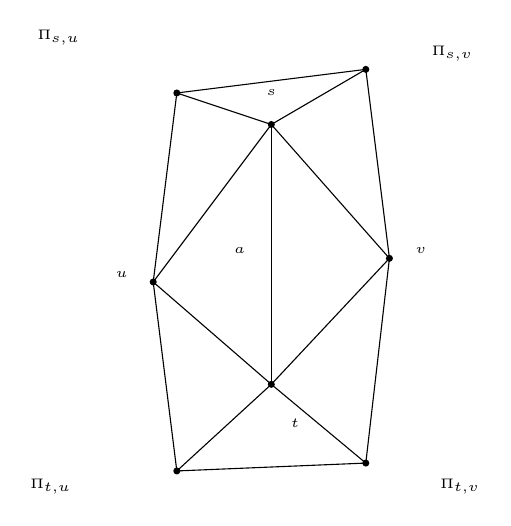
\begin{tikzpicture}[x=1mm,y=1mm,line cap=round,line join=round,font=\scriptsize]
\draw (40,-24) -- (64,-21);
\draw (64,-21) -- (67,-45);
\draw (67,-45) -- (64,-71);
\draw (64,-71) -- (40,-72);
\draw (40,-72) -- (37,-48);
\draw (37,-48) -- (40,-24);
\draw (52,-28) -- (40,-24);
\draw (52,-28) -- (64,-21);
\draw (52,-28) -- (37,-48);
\draw (52,-28) -- (67,-45);
\draw (52,-61) -- (40,-72);
\draw (52,-61) -- (64,-71);
\draw (52,-61) -- (37,-48);
\draw (52,-61) -- (67,-45);
\draw (52,-28) -- (52,-61);
\node[pt] at (40,-24) {};
\node[pt] at (64,-21) {};
\node[pt] at (67,-45) {};
\node[pt] at (64,-71) {};
\node[pt] at (40,-72) {};
\node[pt] at (37,-48) {};
\node[pt] at (52,-28) {};
\node[pt] at (52,-61) {};
\node[inner sep=1pt] at (25,-17) {\tiny $\Pi_{s,u}$};
\node[inner sep=1pt] at (75,-19) {\tiny $\Pi_{s,v}$};
\node[inner sep=1pt] at (24,-74) {\tiny $\Pi_{t,u}$};
\node[inner sep=1pt] at (76,-74) {\tiny $\Pi_{t,v}$};
\node[inner sep=1pt] at (33,-47) {\tiny $u$};
\node[inner sep=1pt] at (71,-44) {\tiny $v$};
\node[inner sep=1pt] at (52,-24) {\tiny $s$};
\node[inner sep=1pt] at (55,-66) {\tiny $t$};
\node[inner sep=1pt] at (48,-44) {\tiny $a$};
\end{tikzpicture}
\end{document}
